\documentclass[10pt,a4paper,oneside]{book}
\usepackage[utf8]{inputenc}
\usepackage[spanish]{babel}
\usepackage{amsmath}
\usepackage{amsfonts}
\usepackage{amssymb}
\usepackage{graphicx}
\usepackage[left=2cm,right=2cm,top=2cm,bottom=2cm]{geometry}
\usepackage{hyperref}
\usepackage{wrapfig}
\hypersetup{
    colorlinks=true,
    linkcolor=cyan,
    anchorcolor=cyan,
    filecolor=cyan,
    urlcolor=blue,
}

%Header and footer customized
\usepackage{fancyhdr}
\pagestyle{fancy}

\usepackage{xcolor}
\usepackage{titling}

\usepackage{listingsutf8}
\usepackage{listings}
\usepackage{color}


%New colors defined below
\definecolor{codegreen}{rgb}{0,0.6,0}
\definecolor{codegray}{rgb}{0.5,0.5,0.5}
\definecolor{codepurple}{rgb}{0.58,0,0.82}
\definecolor{backcolour}{rgb}{0.95,0.95,0.92}

%Code listing style named "mystyle"
\lstdefinestyle{mystyle}{
  backgroundcolor=\color{backcolour},   commentstyle=\color{codegreen},
  keywordstyle=\color{magenta},
  numberstyle=\color{codegray},
  stringstyle=\color{codepurple},
  basicstyle=\scriptsize\ttfamily\tiny,
  breakatwhitespace=false,         
  breaklines=true,                 
  captionpos=b,                    
  keepspaces=true,                                     
  numbersep=5pt,                  
  showspaces=false,                
  showstringspaces=false,
  showtabs=false,                  
  tabsize=2,
  framextopmargin=1pt,
  framexbottommargin=10pt,
}

\usepackage{sectsty}
\partfont{\large}

%"mystyle" code listing set
\lstset{style=mystyle}

%For generate graphs
\usepackage{pgf}
\usepackage{tikz}
\usetikzlibrary{arrows,automata}

% To generate a box with text and background
\definecolor{shadecolor}{RGB}{200,201,190}
\newcommand{\mybox}[1]{\par\noindent\colorbox{shadecolor}
{\parbox{\dimexpr\textwidth-2\fboxsep\relax}{#1}}}

\author{Ruben Vasallo Gonzalez}
\title{PROYECTO FINAL MÁSTER \\ CLASIFICADOR DOCUMENTOS MÉDICOS HOPE \\ 2020 - 2021}

%header
\headsep = 1,5cm
\lhead{\begin{picture}(0,0) \put(0,0){
\includegraphics[width=2cm]{logo-uoc-default.png}} \end{picture}}
\chead{}
\rhead{\thetitle \\ \theauthor}

%footer
\lfoot{}
\cfoot{\thepage}
\rfoot{}

%set head of page
\setlength{\textheight}{230mm}

\begin{document}
\maketitle

\tableofcontents

\iffalse
Notas: (imagen en formato svg), hacer referencia a las imagenes en el texto. si hay mucho codigo, ponerlo en el anexo

mendele

cambiar usuario por profesional sanitario o paciente segun sea el caso, en los objetivos y cambiar mostrar por recomendar.

poner que se hicieron X reuniones para acordar los problemas que existen y como mejorar el analisis (en la extracion de los datos)
enlazar las imagenes con el texto
\fi

\newpage
\chapter{}

\section{Resumen}

\paragraph{}
El proyecto nace de la necesidad de poder disponer de una manera sencilla e inmediata, artículos médicos catalogados según los síntomas de pacientes, pudiendo hacer un \textit{ranking} de más o menos interés en función del \textit{feedback} aportado por los profesionales sanitarios sobre artículos relacionados con esos \textit{síntomas}.

\section{Astract}
TODO

\section{Keywords}

\paragraph{}
clasificador articulos medicos, PCA, KNN, Regresion Logistica, Random Forest, SVM

\newpage
\chapter{Introducción}

\section{Definición del proyecto}
\label{def:def1}

\paragraph{}
El proyecto que aquí se presenta nace de la necesidad por parte del \textit{proyecto HOPE} de clasificar y recomendar resultados sobre estudios clínicos de confianza y que estén actualizados. En Internet existe muchísima información sobre medicina y salud y no siempre toda es de fiar.

\paragraph{}
El proyecto HOPE (que significa \textit{Health Operations for Personalized Evidence} en ingles) nace de la necesidad de ayudar a los profesionales sanitarios a encontrar la información que necesitan de la manera más rápida y fácil posible. Existe infinidad de información medica en Internet de miles de proyectos de investigación medica y esto hace que, muchas veces sea complicado encontrar la información sobre ensayos médicos para tratar información. En el ámbito de la medicina el tiempo perdido puede costar vidas y es un precio demasiado elevado a pagar, tanto a nivel económico como emocional.

\paragraph{}
Actualmente existen bases de datos de confianza en donde los profesionales sanitarios y el publico en general puede buscar informes y ensayos sobre estudios clínicos desarrollados anteriormente, pero no siempre es fácil o rápido encontrar estos resultados.

\paragraph{}
El proyecto HOPE es un sistema basado en inteligencia artificial para identificar los datos claves de casos clínicos registrados en la Historia Clínica Electrónica, en base a los cuales realiza una búsqueda única por paciente para proporcionar al profesional sanitario recomendaciones de tratamientos, estudios de investigación, información para el paciente, todo en base a registros de fuentes científicas de información. En este proyecto, profesionales sanitarios de todo el mundo puede consultar en una base de datos informes médicos relacionados con los síntomas que puedan tener sus pacientes y ver que otros tratamientos han dado resultado. Todo y con eso, el sistema no siempre devuelve los artículos más relevantes o actualizados por lo que, no siempre la información consultada es útil.

\paragraph{}
En este ámbito, los profesionales sanitarios pueden valorar si la información recibida ha sido útil o no respecto a la búsqueda que han realizado, por lo que con ese \textit{feedback}, se pretende mejorar el sistema actual complementándolo con un modelo clasificador capaz de ayudar al actual a entregar realmente los artículos útiles basándose en el \textit{feedback} que los profesionales sanitarios dan al sistema.


\section{Estado del arte}
Recomendadores que existen actualmente:


\chapter{Objetivos del Máster}

\section{Objetivo principal}

\label{op:OP1}
\paragraph{OP} - Poder recomendar al profesional sanitario cuales son los artículos más útiles que pueden ayudar en el tratamiento del paciente, en base a los síntomas que este tiene, pudiendo realizar un \textit{ranking} de mas interés a menos.

\section{Objetivos secundarios}

\paragraph{}
Para poder cumplir con el objetivo principal \hyperref[op:OP1]{OP1}, desglosaremos los siguientes objetivos secundarios:

\label{os:OS1}
\paragraph{OS1} - Extraer la información de la base de datos y tratarla para quedarnos solo con la que consideramos valida.

\label{os:OS2}
\paragraph{OS2} - Hacer un análisis de componentes principales (estudio de que atributos son relevantes para alcanzar el objetivo).

\label{os:OS3}
\paragraph{OS3} - Enriquecer de los datos (\textit{data augmentation}) prediciendo los resultados que no están indicados si son relevantes o no. Aproximación por Vecinos más próximos (\textit{K-Nearest-Neighbor}).

\label{os:OS4}
\paragraph{OS4} - Predecir los resultados usando el algoritmo de aprendizaje supervisado para clasificación llamado Regresión logística "\textit{Logistic regression}".

\label{os:OS5}
\paragraph{OS5} - Predecir los resultados usando el algoritmo de aprendizaje supervisado para clasificación llamado Bosques Aleatorios "\textit{Random Forests}".

\label{os:OS6}
\paragraph{OS6} - Predecir los resultados usando el algoritmo de aprendizaje supervisado para clasificación llamado Máquinas de vector soporte "\textit{Support Vector Machines}".

\chapter{Metodología}

\section{Reuniones con el cliente}

\paragraph{}
Para poder comprender y abordar con éxito el \hyperref[op:OP1]{objetivo principal} se realizaron 4 reuniones en donde el cliente expuso el \hyperref[op:OP1]{problema} a abordar y el origen de los datos para poder realizar el estudio.

\paragraph{}
En estas reuniones se pudo observar que los datos facilitados por el usuario requerían de una limpieza y tratamiento para poder cumplir el objetivo principal, ya que muchas observaciones tenían información poco relevante que podía generar ruido.

\paragraph{}
Realizando un primer análisis visual, se detecto que los datos aportados por el cliente eran insuficientes para completar el \hyperref[op:OP1]{OP1}, ya que solo se disponía de la información respecto de si un articulo había sido útil o no, pero no se disponía de la información suficientemente detallada para saber si había sido muy útil o poco útil para poder llegar a realizar un \textit{ranking}. El cliente nos comenta que en el momento actual no dispone de ese nivel de detalle y se acuerda con el que, se realizara una aproximación para indicar si un articulo es útil o no dejando para mas adelante la opción de poder realizar \textit{rankins} si se consigue ese nivel de detalle por parte del cliente.

\paragraph{}
También se pudo comprobar que el cliente disponía de un volumen de observaciones bajo por lo que se planteo la posibilidad de, o intentar obtener más observaciones facilitadas por el cliente, o intentar enriquecer las observaciones actuales generando nuevos datos por aproximación a los reales.

\paragraph{}
Finalmente se decidió estudiar si era viable generar nuevos valores por aproximación, debido a que en el momento en que se trato el problema, el cliente no podía facilitar más datos. Si a lo largo del estudio, el cliente conseguía facilitar nuevas observaciones, estas serian añadidas al estudio para aproximar mejor la solución final.

\section{Extracción de los datos}

\paragraph{}
Para cumplir con el \hyperref[op:OP1]{OP1} mostramos los pasos que hemos seguido para extraer y procesar los datos:

\paragraph{}
El Origen de los datos se encuentra en una Base de datos SQL distribuida en dos tablas, que pasamos a detallar a continuación:

\paragraph{}
En la primera tabla llamada \textit{fed\_hope\_sugerencia}, encontraremos la sugerencia que dio el programa HOPE en base a los parámetros que introdujo el profesional sanitario, almacenado en el atributo pedido y la respuesta que dio el programa, almacenado en el atributo respuesta. Todos los datos son almacenados en formato documento json.

\paragraph{}
En la figura \ref{tablaFedHopeSugerencia} mostramos los atributos de la tabla \textit{fed\_hope\_sugerencia}.

\paragraph{}
\begin{figure}[!htb]
  \centering
    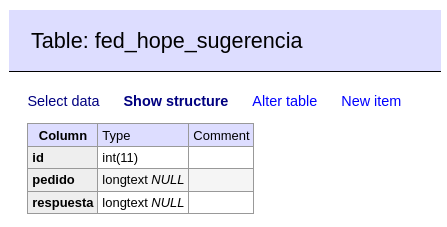
\includegraphics[width=8cm]{images/metodologia_tabla_fed_hope_sugerencia.png}
    \caption{Visualización de los atributos de la tabla \textit{fed\_hope\_sugerencia}}
  \label{tablaFedHopeSugerencia}
\end{figure}

\paragraph{}
Si analizamos el \textbf{atributo pedido}, podemos observar, tal y como se muestra en la figura \ref{atributoPedido}, varios atributos haciendo referencia a los síntomas que consulta el profesional sanitario.

\begin{figure}[!htb]
  \centering
    \lstset{inputencoding=utf8/latin1}
    \lstinputlisting[frame=single]{codes/metodologia_tabla_fed_hope_sugerencia_attribute_pedido.json}
    \caption{Muestra de una observación del atributo pedido}
  \label{atributoPedido}
\end{figure}

\paragraph{}
Si analizamos el \textbf{atributo respuesta}, podemos observar entre otros datos, el listado de artículos médicos sugeridos relacionados con los síntomas descritos por el profesional sanitario. Esta respuesta es muy amplia pero entre todos los atributos, podemos observar un listado de identificadores de artículos, con sus fechas de revisión de estos, y unas palabras claves descriptivas para esos artículos.

\paragraph{}
A continuación mostramos en la figura \ref{atributoRespuesta} una pequeña parte del contenido de una observación del atributo respuesta.
\begin{figure}[!htb]
  \centering
    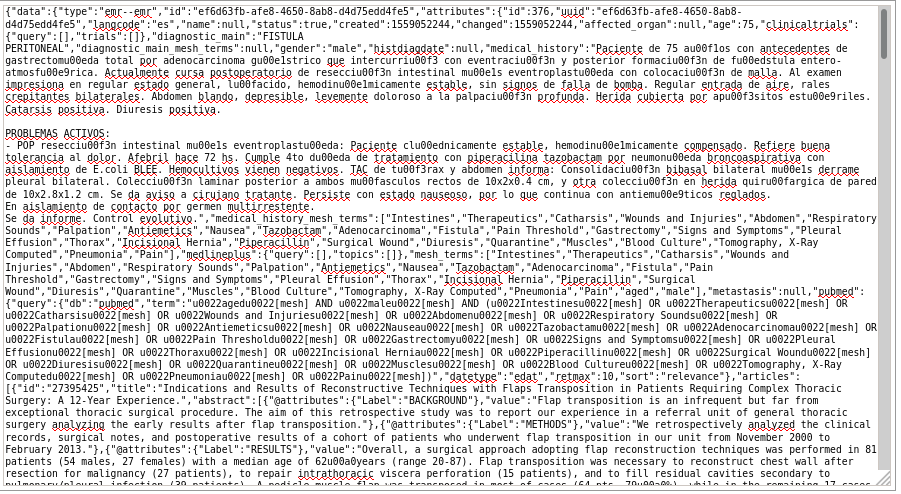
\includegraphics[width=15cm]{images/metodologia_tabla_fed_hope_sugerencia_attribute_respuesta.png}
    \caption{Ejemplo de contenido del atributo respuesta de una observación}
  \label{atributoRespuesta}
\end{figure}

\newpage
\paragraph{}
En la segunda tabla llamada \textit{fed\_hope\_sugerencia\_feedback}, encontraremos, tal y como se muestra en la figura \ref{tablaFedHopeSugerenciaFeedback}, la opinión \textit{feedback} (que utilidad ha tenido la información por parte del profesional sanitario) de la información recibida dado un articulo en concreto en una búsqueda en concreto. Esta información se relaciona con la tabla \textit{fed\_hope\_sugerencia} a través del atributo \textit{fed\_hope\_sugerencia\_id}.

\paragraph{}
En esta tabla, esta representada la opinión \textit{feedback} del profesional sanitario en el atributo \textit{utilidad}, que denota un valor 0 para los artículos que han sido poco útiles respecto a la búsqueda realizada y 1 para los artículos que si han sido útiles.

\paragraph{}
\begin{figure}[!htb]
  \centering
    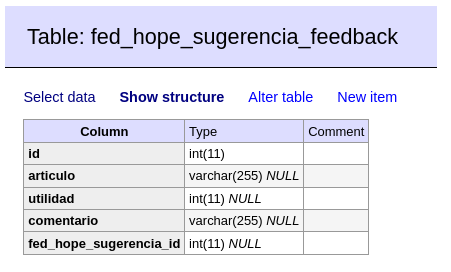
\includegraphics[width=8cm]{images/metodologia_tabla_fed_hope_sugerencia_feedback.png}
    \caption{Visualización de los atributos de la tabla \textit{fed\_hope\_sugerencia\_feedback}}
  \label{tablaFedHopeSugerenciaFeedback}
\end{figure}

\paragraph{}


\newpage
\subsection{Lectura de los datos}

\paragraph{}
Para extraer los datos de la base de datos nos ayudaremos de las librerías \textit{sqlalchemy} y \textit{pymysql} programadas en lenguaje \textit{python} que nos permitirá acceder a la información almacenada en una base de datos \textit{MySQL} y devolvérnosla en formato \textit{dataframe}, un formato que nos permite entre otras cosas, realizar transformaciones de los datos para conseguir nuestro objetivo final.

\paragraph{}
Este formato es interpretable por la librería \textit{pandas} y \textit{numpy}, dos librerías programadas en lenguaje \textit{python}, muy comunes en el ámbito de la ciencia del dato, que nos facilitara entre otras cosas, poder hacer operaciones matemáticas con los datos de manera eficiente. A continuación mostramos en la figura \ref{readDataBD} el código utilizado para extraer los datos de la tabla \textit{fed\_hope\_sugerencia}.

\paragraph{}
\begin{figure}[!htb]
  \centering
    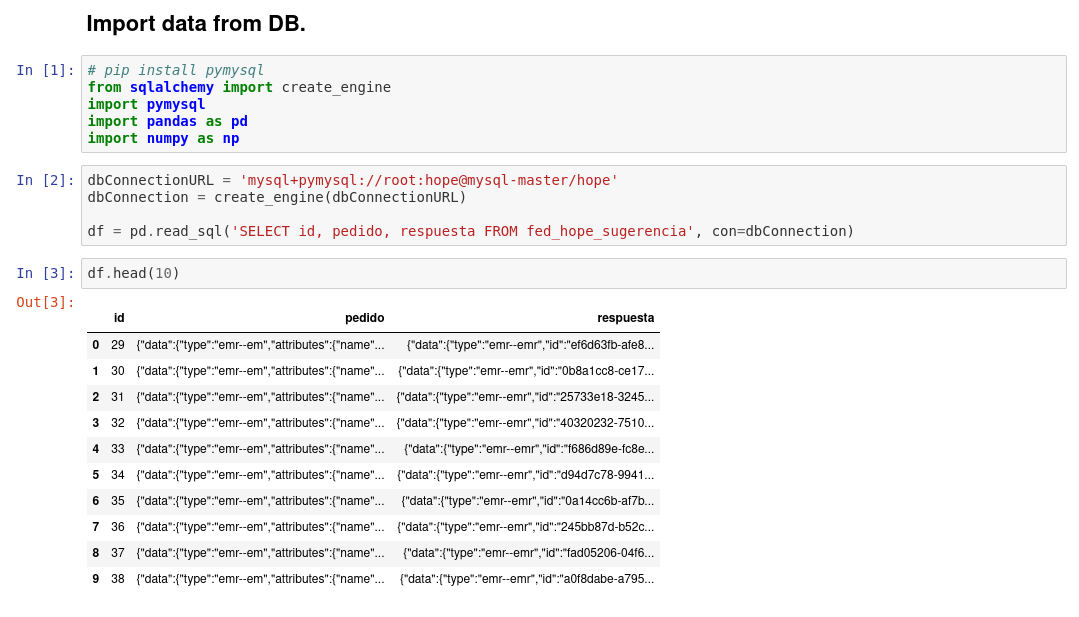
\includegraphics[width=0.9\textwidth]{images/metodologia-extract-data-mysql.png}
    \caption{Lectura de los datos}
  \label{readDataBD}
\end{figure}

\paragraph{}
Aplicaremos los mismos pasos para leer la información del feedback de los profesionales sanitarios de la tabla \textit{fed\_hope\_sugerencia\_feedback}

\newpage
\subsection{Conversión a formato columnar}

\paragraph{}
Para poder trabajar con los datos, necesitaremos que estos estén en formato columnar (tabla relacional) por lo que necesitaremos convertir los datos de estos \textit{json} en tablas relacionales (A esta acción se le conoce como \textit{flattening} o aplanar). 

\paragraph{}
Este paso consiste en coger cada uno de los atributos que tiene el json y convertirlos en columnas de una tabla, añadiendo los valores. Si el \textit{json} tiene varios niveles, este proceso añadirá tantas columnas como niveles tenga el \textit{json}, siempre que todas las observaciones del \textit{json} tengan el mismo formato. Este caso se nos cumple para las observaciones del atributo Pedido. No es así para las observaciones del atributo respuesta en el que tendremos que hacer un tratamiento especial que detallaremos posteriormente.

\paragraph{}
Cuando se analizan los datos recuperados, se detecta que estos, contienen caracteres que informan de los saltos de linea o tabulacion. Estos caracteres pueden ser mal interpretados a la hora de leer los datos de los documentos en formato \textit{json} por lo que sera necesario eliminarlos.

\paragraph{• \textit{Flattening} del atributo pedido}

\paragraph{}
Para realizar la acción de \textit{flattening} en el atributo pedido, nos ayudaremos de la funcionalidad \textit{json\_normalize} del paquete pandas que realiza esta acción. A continuación mostramos en la figura \ref{flatteningPedido} el código utilizado para el atributo pedido.

\paragraph{}
\begin{figure}[!htb]
  \centering
    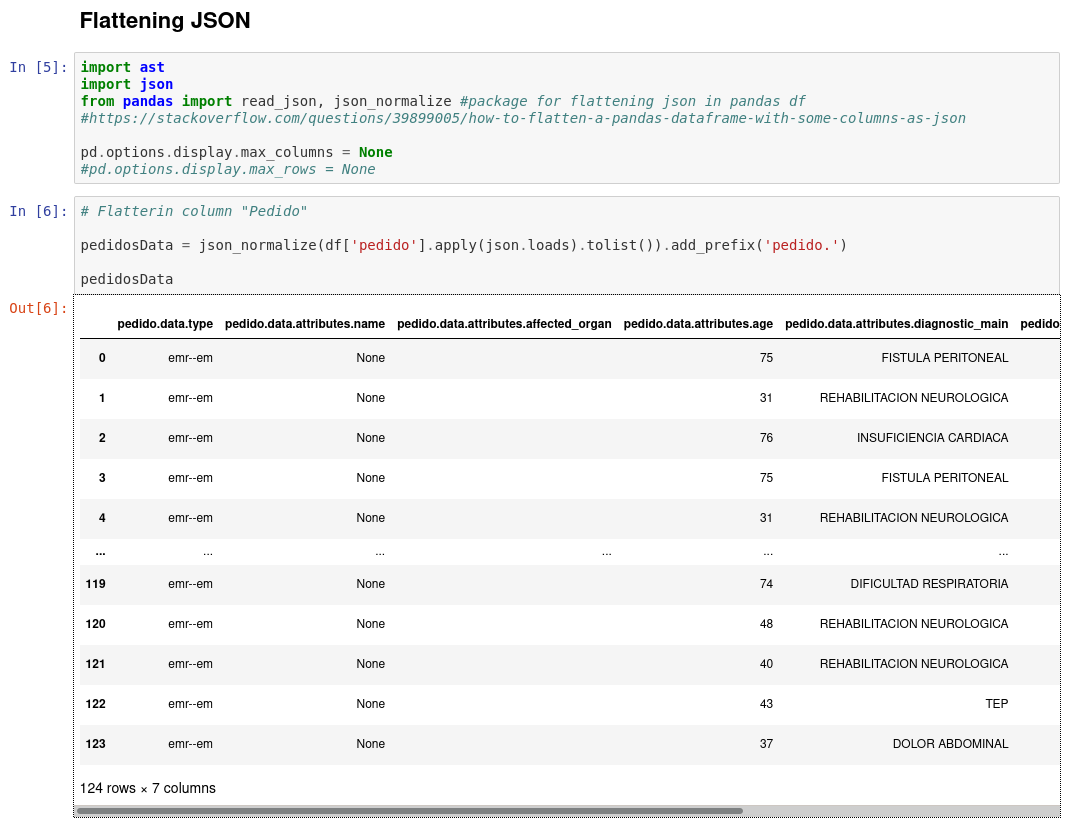
\includegraphics[width=0.9\textwidth]{images/metodologia-aplanar-pedido.png}
    \caption{\textit{Flattening} del atributo pedido.}
  \label{flatteningPedido}
\end{figure}

\paragraph{• \textit{Flattening} del atributo respuesta}

\paragraph{}
Debido a que la información almacenada en el documento \textit{json}, en el atributo respuesta es muy compleja (debido a que esta contiene diferentes documentos con diferentes niveles de información) como se puede apreciar en el apartado X, no podemos aplanar la información directamente como hemos hecho con el atributo pedido. Por lo que tenemos que analizar que información nos interesa recoger para enriquecer el dataset de datos.

\paragraph{}
Después de analizar el documento, y ayudarnos del conocimiento del cliente, vemos que los atributos más interesantes son los que hacen referencia al identificador del articulo, las palabras claves asociadas al articulo por parte de la api pubmed y el mes y año de la revisión del articulo. Para recoger esta información nos crearemos una función que acceda directamente a estos atributos dado una observación. Después ejecutaremos esa función para cada observación ayudándonos de la función \textit{apply}. A continuación mostramos este proceso en la figura \ref{flatteningRespuesta}.

\paragraph{}
\begin{figure}[!htb]
  \centering
    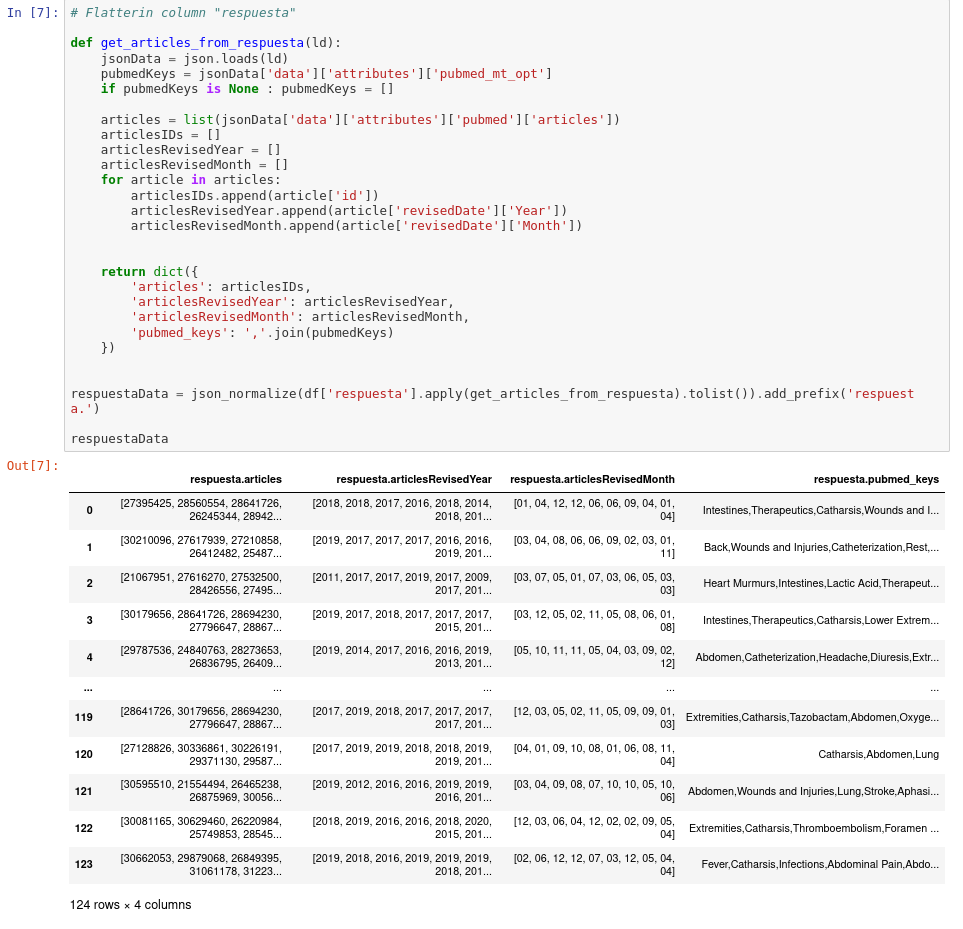
\includegraphics[width=0.9\textwidth]{images/metodologia-aplanar-respuesta.png}
    \caption{\textit{Flattening} del atributo respuesta.}
  \label{flatteningRespuesta}
\end{figure}

\paragraph{}
Una vez aplanado los dos atributos, los uniremos en un único dataset junto a los datos originales de la tabla \textit{fed\_hope\_sugerencia} para poder trabajar con ellos. Estos es importante para mantener el id de cada observación, de cara a poder luego identificar el feedback de los profesionales sanitarios con cada observación.

\newpage
\section{Procesado de los datos}

\subsection{Análisis de los datos}
Una vez tenemos los datos en formato tabular, observamos que existen ciertos atributos que contienen listas de opciones como son los atributos \textit{pubmed\_keys} (que corresponde a las palabras clave que la api de pubmed nos devuelve para esta observación), \textit{articles} (que corresponde a los ids de los artículos relacionados con esa observación), \textit{articlesRevisedYear} i \textit{articlesRevisedMonth} (que corresponde a los años y meses de los artículos según están ordenados en el atributo \textit{articles})

\paragraph{}
Como nuestro \hyperref[op:OP1]{OP1} es poder recomendar artículos útiles, necesitamos tener una observación por articulo, para poder posteriormente analizar de manera independiente si ese articulo fue útil o no para la observación a la que hace referencia.

\paragraph{}
Por lo que necesitaremos expandir (duplicar) cada observación con solo un articulo que haga referencia a el. A continuación mostramos en la figura \ref{expandArticles} el código para expandir el atributo \textit{articles} (el resto de atributos su proceso seria similar).

\paragraph{}
\begin{figure}[!htb]
  \centering
    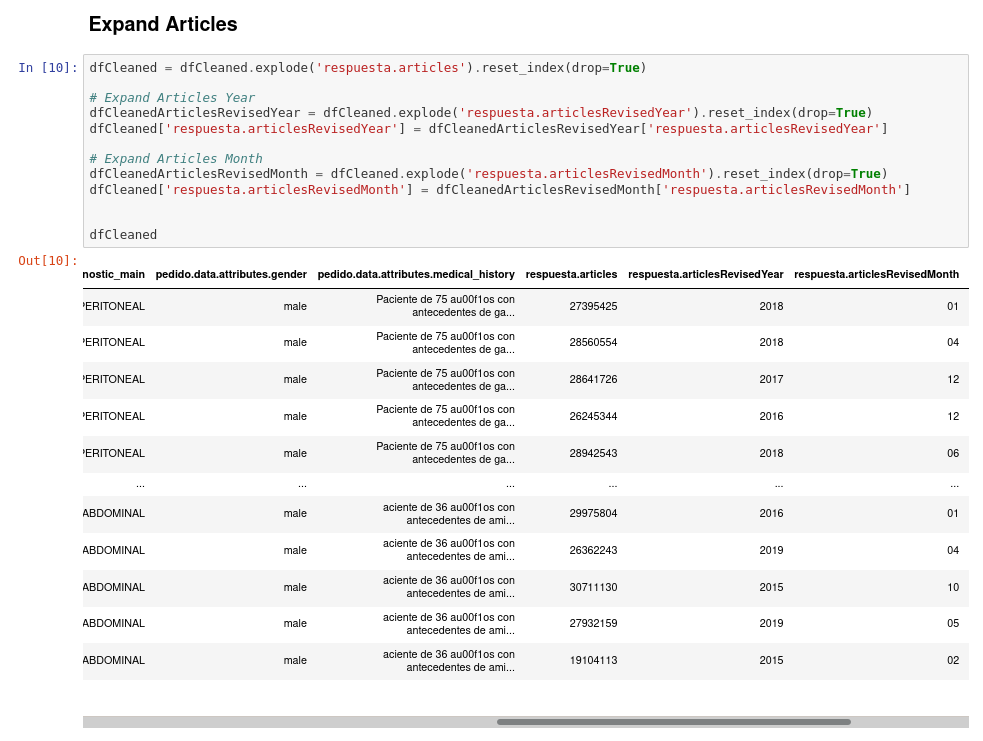
\includegraphics[width=0.9\textwidth]{images/metodologia_procesado_de_datos_expandir_articulos.png}
    \caption{Expansión del atributo \textit{articles}.}
  \label{expandArticles}
\end{figure}

\paragraph{}
Después de tener un articulo por observación, observamos que tenemos atributos poco relevantes (como el atributo \textit{data.type} o \textit{Name} que contiene siempre el mismo valor) o que no contienen información alguna (como el atributo \textit{affected\_organ}) como se puede observar en la figura \ref{atributesEmpty}. Eliminaremos estos atributos junto a otros con la misma casuistica, para no generar ruido en el posterior análisis predictivo.

\paragraph{}
\begin{figure}[!htb]
  \centering
    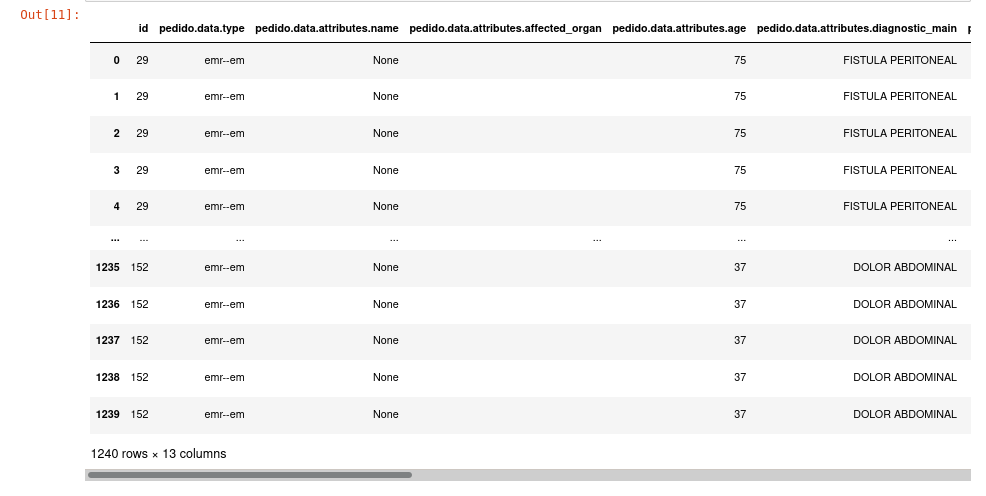
\includegraphics[width=0.9\textwidth]{images/metodologia_analisis_datos_atributos_sin_valor.png}
    \caption{Se detectan algunos atributos con poca o nula relevancia.}
  \label{atributesEmpty}
\end{figure}

\paragraph{}
Y con estos pasos hemos cubierto el \hyperref[os:OS1]{OS1}

\newpage
\subsection{Análisis de componentes principales}
TODO

\newpage
\section{Enriquecimiento de los datos. Aproximación por Vecinos más próximos (K-NN)}
TODO

\newpage
\section{Modelos Predictivos}

\subsection{Regresión logística \textit{'Logistic regression'}}
TODO

\subsection{Bosques Aleatorios \textit{'Random Forest'}}
TODO

\subsection{Maquinas de Vector Soporte \textit{'Support Vector Machines'}}
TODO

\newpage
\section{Resultados}
TODO

\newpage
\chapter{Conclusiones}
TODO

\chapter{Bibliográfica}

\cleardoublepage
\phantomsection
\addcontentsline{toc}{chapter}{\listfigurename}
\listoffigures

\chapter{Anexos}

\end{document}